\section{Service Contract Notations}
A Service contract refers to the definition of a service provided by an application component, detailing its inputs, outputs, and behavior. A service contract is a fundamental building block of service-oriented architecture (SOA), and serves as a shared understanding between the provider and consumer of the service. Examples of Service Contract notations are: OpenAPI, gRPC, Web Service Description Framework, Representational State Transfer.

\subsection{OpenAPI}
The OpenAPI specification (OAS), formerly known as the Swagger specification, is a format for describing RESTful APIs. It uses a simple YAML or JSON file to describe the structure of an API, including its endpoints, input and output parameters, authentication methods, and other information. The specification can be used to generate documentation, client libraries, and other tools that make it easier to consume and work with an API. It is widely supported and has a large ecosystem of tools and libraries built around it.

\begin{figure}[H]
  \center
  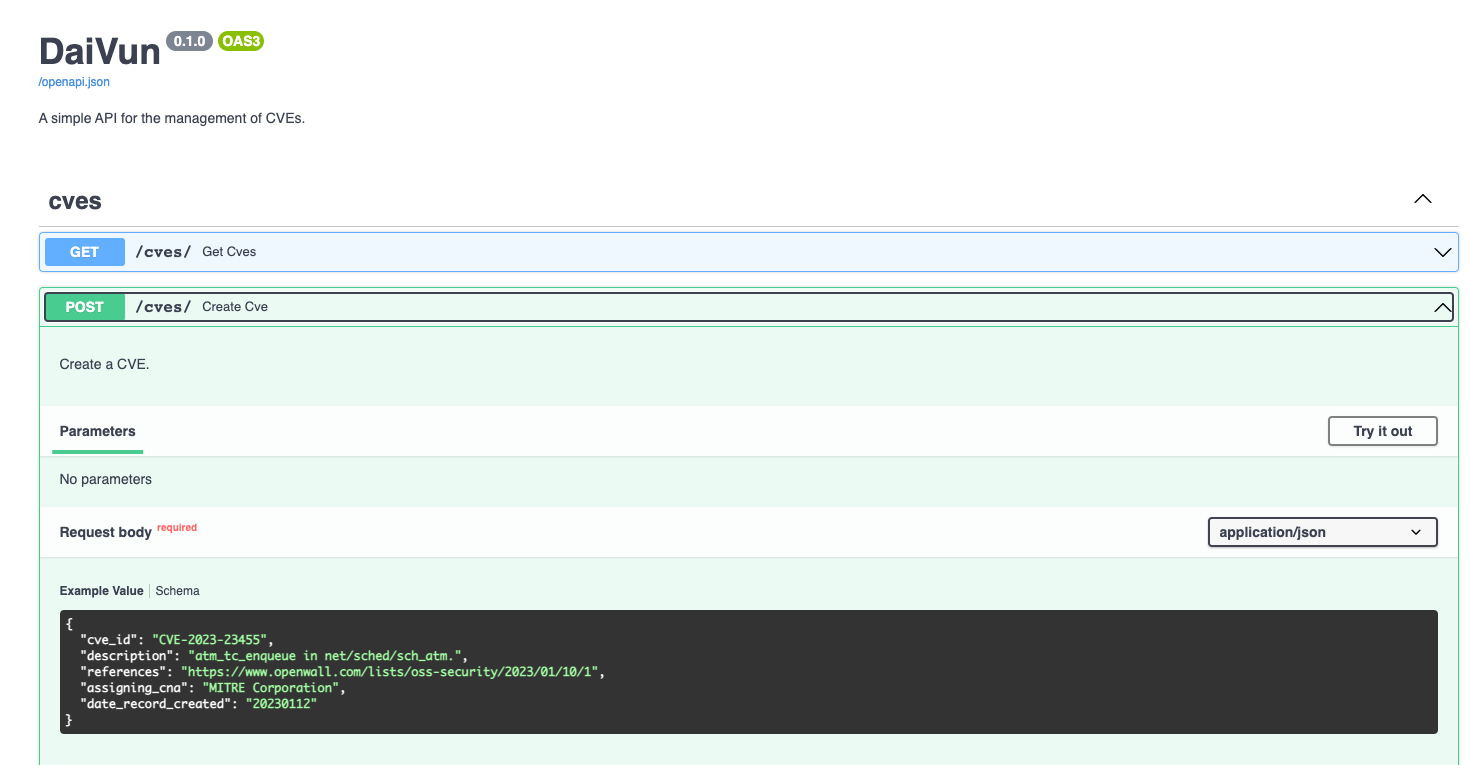
\includegraphics[width=\textwidth]{openapi}
  \caption{OpenAPI Example Documentation}
\end{figure}

\subsection{Web Service Description Language (WSDL)}
The Web Service Description Language (WSDL) is an XML-based language used to describe the functionality offered by a web service. It defines the operations (methods) that can be called on the service, the inputs and outputs for those operations, and the location of the service (the endpoint). 

\subsection{Microservice Domain-Sepcific Language (MSDL)}
Microservice Domain-Specific Language (MDSL) is a language specifically designed to describe the structure and behavior of microservices. It is used to define the interface, dependencies, and other aspects of a microservice, and can be used to generate code, documentation, and other artifacts.

\section{Microservice API Patterns (MAPI)}
Microservice API Patterns (MAPI) refer to a set of best practices and design patterns for building and exposing APIs in a microservice architecture. MAPI helps ensure that APIs are consistent, scalable, secure, and easily consumable by clients.

\begin{figure}[H]
  \center
  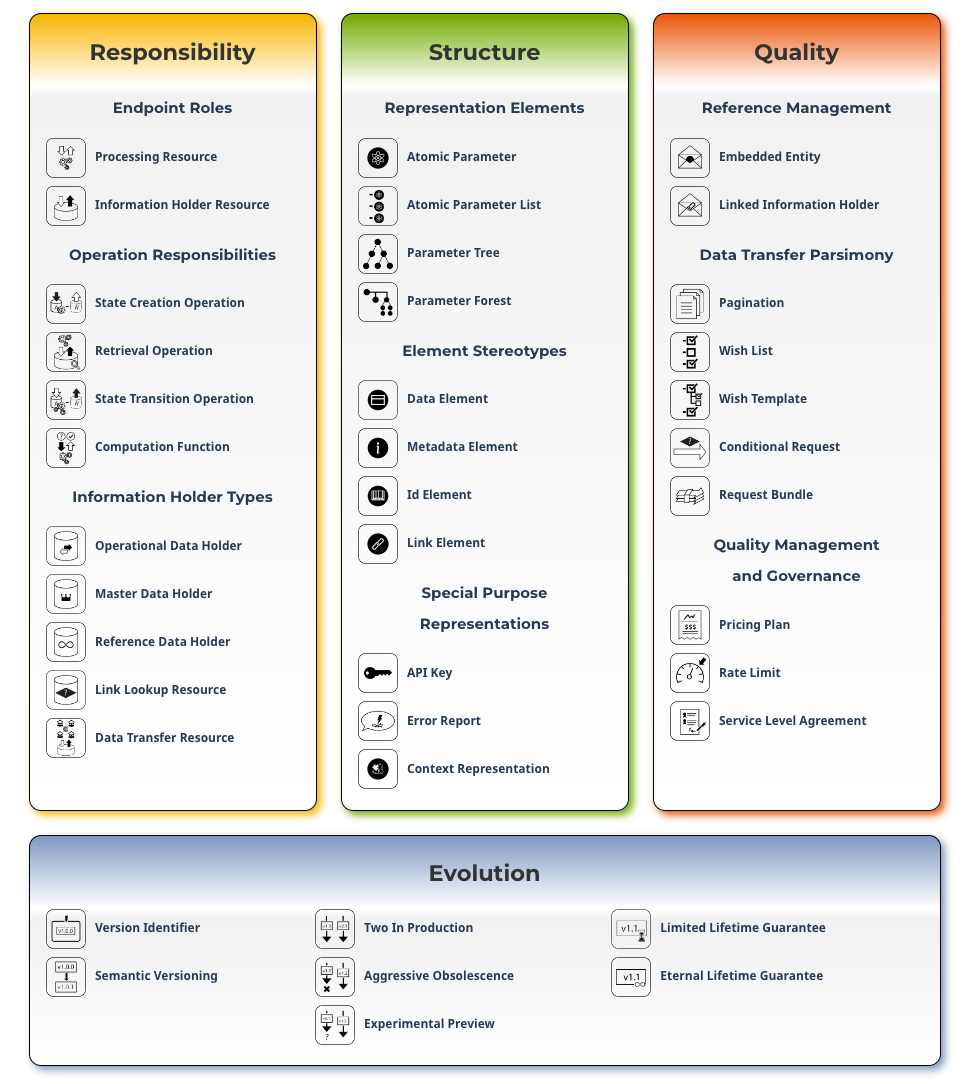
\includegraphics[width=\textwidth]{mapi}
  \caption{Mircoservice API Patterns}
\end{figure}